\documentclass[amsmath,preprintnumbers,10pt,nofootinbib,prl,twocolumn]{revtex4-1}
\usepackage{amsbsy}
\usepackage{amssymb}
\usepackage{graphicx}
\usepackage{color}
\usepackage{subfigure}
\usepackage{physics}
\usepackage{soul}
\usepackage{color}
\usepackage{bm}
\usepackage[normalem]{ulem}

%\newcommand{\Tr}{\text{Tr}}
\newcommand{\Ai}{\text{Ai}}
\newcommand{\Bi}{\text{Bi}}
\newcommand{\Real}{\text{Re}}
\newcommand{\Imag}{\text{Im}}

\usepackage{verbatim}
\usepackage{natbib}
\bibliographystyle{apsrev4-1}
\begin{document}
\title{Dissipation induced transitions in two dimensional elastic membranes}
\author{Michael Nguyen$^{1,2}$, Suriyanarayanan Vaikuntanathan$^{1,2}$} 
\affiliation{$^1$The James Franck Institute, The University of Chicago, Chicago, IL,}
\affiliation{$^2$ Department of Chemistry, The University of Chicago, Chicago, IL.}
\begin{abstract}
Stochastic thermodynamics provides a useful set of tools to analyze and constrain the behavior of far from equilibrium systems. In this paper, we report an application of ideas from stochastic thermodynamics to the problem of membrane growth. Non-equilibrium forcing of the membrane can cause it to buckle and undergo a morphological transformation. We show how ideas from stochastic thermodynamics, in particular the recently derived thermodynamic uncertainty relations, can be used to phenomenologically describe and constrain the parameters required to excite morphological changes during a non-equilibrium growth process.

\end{abstract}
\maketitle 


\noindent{\it Introduction:} Non-equilibrium forcing can be used to uncover new strategies for self-assembly and organization~\cite{Battle604,Lan2012,Mehta2012,Whitelam2014}. In biophysical contexts, it has been established that non-equilibrium forces play a crucial role in suppressing rogue fluctuations and enhancing fidelity of molecular recognition~\cite{Hopfield1974,Mehta2012,Murugan2012,Murugan2016,Vaikunt2017}, support robust oscillations crucial for the maintenance of circadian rhythms~\cite{Barato2017}, and drive sensory adaptation processes~\cite{Lan2012,Mehta2012}. Non-equilibrium forces also play an important role in modulating cell shape and cell membrane fluctuations~\cite{McMahon2005, Turlier2016}. For instance, local changes in surface tension or lateral pressure due to a spontaneous assembly of membrane proteins have been known to induce instabilities in membrane fluctuations~\cite{Stachowiak2012, Chen2016,Rangamani2014,Leibler1986}. Such instabilities have been implicated as important precursors during cell division~\cite{McMahon2005}. Non-equilibrium fluctuations are also important in cases where the cell membrane interacts with growing actin filaments. The important role played by such interactions in regulating the organization of the membrane has been well established ~\cite{Gowrishankar2012,Weichsel2016}.
\begin{figure}[tbb]
\centering
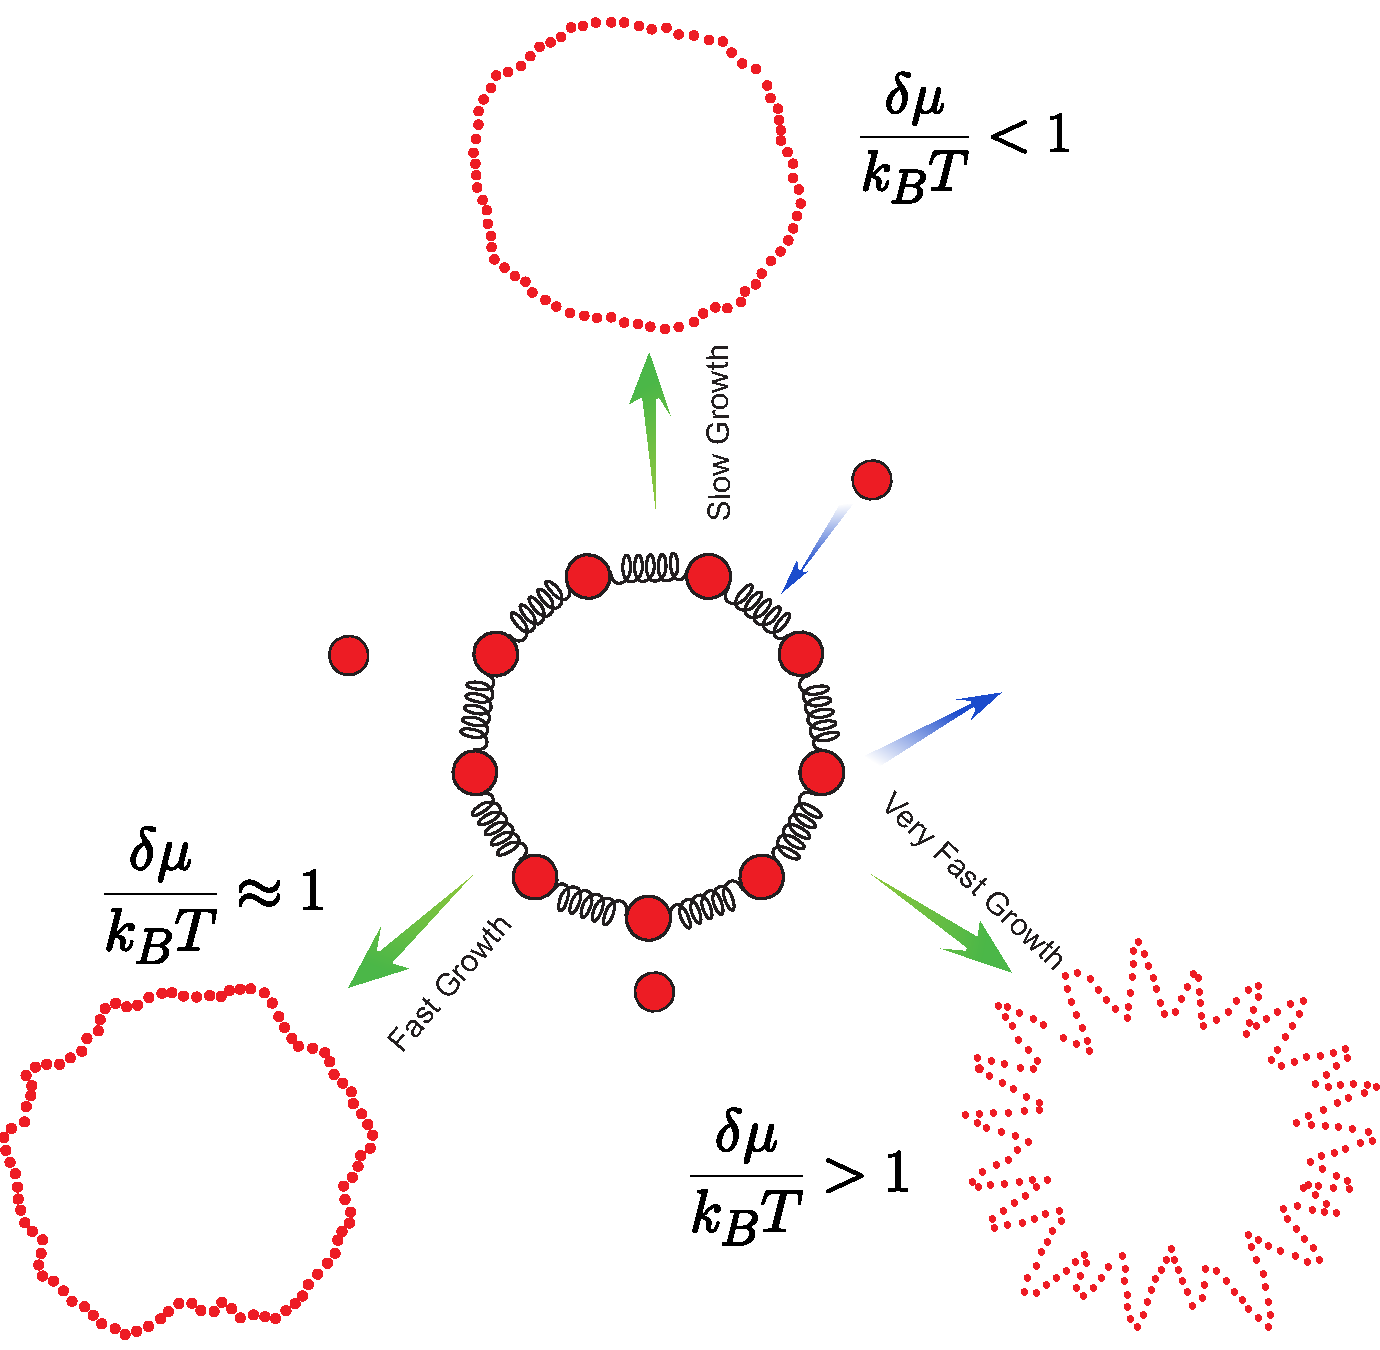
\includegraphics[scale=0.35]{Fig1.pdf}
\caption{Schematic of the growing assembly. When the assembly grows slowly, its shape remains circular (top figure). As the assembly grows faster, its shape becomes more distorted (lower left) and ultimately it buckles into a star-shaped morphology (lower right). We have included movies in the SI showing this transformation.} \label{fig:phases}
\end{figure}

%In particular, the field of stochastic thermodynamics has provided a promising framework to study non-equilibrium systems in mesoscopic scale~\cite{Seifert2012}. The ideas of stochastic thermodynamics have been productively used to elucidate tradeoffs between energy consumption and organization in biochemical reaction networks~\cite{Barato2015,Murugan2016,Vaikunt2017}, self-propelled or driven colloids~\cite{Ganguly2013, delJunco2018,Dasbiswas2017}, and molecular motors~\cite{Gaveau2010, Seifert2011}. Previously, we have also shown how stochastic thermodynamics can be used to derive general design principles for self-assembly~\cite{Nguyen2016}. 
%In particular, our central results show how an application of stochastic thermodynamics to such systems can provide bounds on the parameters required to renormalize material properties and excite morphological transformations in the membrane system. Our bounds are thermodynamic in nature and depend minimally on the kinetic details of the process chosen (Eqs.~\ref{eq:firstbound} and \ref{eq:secondbound} below). While a detailed kinetic model can indeed be written down to explain the phenomenology observed in our model non-equilibrium growth simulations, the utility of a thermodynamic bound is that it can identify combinations of parameters that remain important for reorganization irrespective of kinetic details. As such, we anticipate that our work will be useful for uncovering minimum sets of energetic requirements for driving more complex classes of reorganization events in model membrane systems~\cite{Zwicker2017}. 

% The interactions between particles are chosen such that the fluctuations of the ring at equilibrium can be described by specifying a surface or a line tension and a bending rigidity.

%who used this model to gain more insights into membrane behaviors.  Their paper then inspired many following papers~\cite{Fisher1989a,Rudnick1991,Rajesh2008,Nelson2009} which use similar models to study membranes with both analytical results and simulations.} Despite its apparent simplicity, this elastic model possesses many features

However, unlike the behavior and characteristics of equilibrium systems, general principles governing self-assembly and organization away from equilibrium remain to be discovered. In this letter, we use the framework of stochastic thermodynamics to investigate non-equilibrium growth and morphological changes~\cite{Drasdo2000, Ramaswamy2000,Rao2001,Solon2006,Hannezo2011,Fisher1989,Fisher1989a,Rudnick1991,Rajesh2008,Nelson2009,Mahadevan2019,Wolde2019} in a model elastic membrane (Fig.~\ref{fig:phases}). Our model consists of two-dimensional particles connected by elastic springs in a ring like geometry (Fig~\ref{fig:phases})~\cite{Fisher1989,Fisher1989a,Rudnick1991,Rajesh2008,Nelson2009}. The ring assembly is allowed to exchange particles with a reservoir. The chemical potential of the reservoir controls the growth rate of the ring assembly and sets the non-equilibrium driving force in this system. This elastic model is adapted from an equilibrium model first introduced by Leibler and coworkers in Ref~\cite{Fisher1989}. As demonstrated in Refs~\cite{Fisher1989,Fisher1989a,Rudnick1991,Rajesh2008,Nelson2009}, despite their apparent simplicity, this class of elastic models possess many features~\cite{W.Helfrich1973,Fisher1989,Fisher1989a,Rudnick1991,Ramaswamy2000,Rao2001,Solon2006,Rajesh2008,Hannezo2011,Loubet2012,Nelson2009} characteristic of three-dimensional membranes and can be used to obtain insights into how morphological changes in such systems can be excited under a non-equilibrium driving force.

Indeed, as we describe below, our numerical analysis shows that the effective surface tension and bending rigidity of the elastic ring get modified under non-equilibrium growth conditions. Further, beyond a critical chemical potential driving force, the effective surface tension of the elastic ring is renormalized to zero and the elastic ring exhibits a buckling instability and undergoes a non-equilibrium morphological transformation (Fig.~\ref{fig:phases}). Such instabilities have been observed in experiments investigating the growth of model lipid membranes \cite{Solon2006} and can potentially have implications for biophysical processes such as membrane fission and endocytosis. We note that phenomenology similar to that described above can be observed in three-dimensional elastic membrane models (see SI Sec: 8~\cite{Supplementary}).
% Usually, to understand these membrane's behaviours, we would have to write down hydrodynamics equations such as mass transfer and momentum transfer. However, in this letter, we would like to propose another approach using the principles of thermodynamics to write down thermodynamics bounds with relative ease that can be used to predict the renormalization of the surface tension of the membrane by non-equilibrium drive.

Using ideas from stochastic thermodynamics, we provide a thermodynamic prescription for how the surface tension and bending rigidity are modified by the non-equilibrium forces (Eqs.~\ref{eq:firstbound} and~\ref{eq:secondbound}). The thermodynamic prescription only requires information about the magnitude of the non-equilibrium chemical potential driving force, the equilibrium surface tension and bending rigidity, the average rate of growth, and fluctuations in the growth rate and is otherwise independent of the kinetic details of the growth process. The thermodynamic prescription is otherwise insensitive to any of the kinetic details used in the growth process and provides bounds on the energetic requirements to induce morphological transformations such as the above-described non-equilibrium buckling transition (Fig.~\ref{fig:PhaseDiagram}). 
Eq.~\ref{eq:secondbound} in particular is an adaptation of the recently derived thermodynamic uncertainty relations~\cite{Gingrich2016} to the problem of membrane growth.

A detailed proof for Eq.~\ref{eq:firstbound} and Eq.~\ref{eq:secondbound} is provided in SI Sec: 6~\cite{Supplementary}. This detailed proof shows how ideas like the thermodynamic uncertainty relation~\cite{Gingrich2016,Barato2015}\textendash these have typically been derived for Markov state models with a finite fixed number of states \textendash can be adapted and applied to non-equilibrium membrane growth problems. From this detailed proof, we also anticipate that the central thermodynamic result is not specific to the two-dimensional elastic membrane model and can be applied more broadly to study growth induced morphological transitions in three dimensional membranes (SI Sec: 8~\cite{Supplementary})~\cite{Mahadevan2019}. 
Together, our results form a set of design principles for controlling morphologies and material properties of membranes even in far from equilibrium conditions.

%We hope these results will elucidate the energy requirements for achieving processes reminiscent of cell division in biology and will also clarify how non-equilibrium forces can be used as an effective knob for tuning fluctuations in many body condensed systems.

\begin{figure}[tbb]
\centering
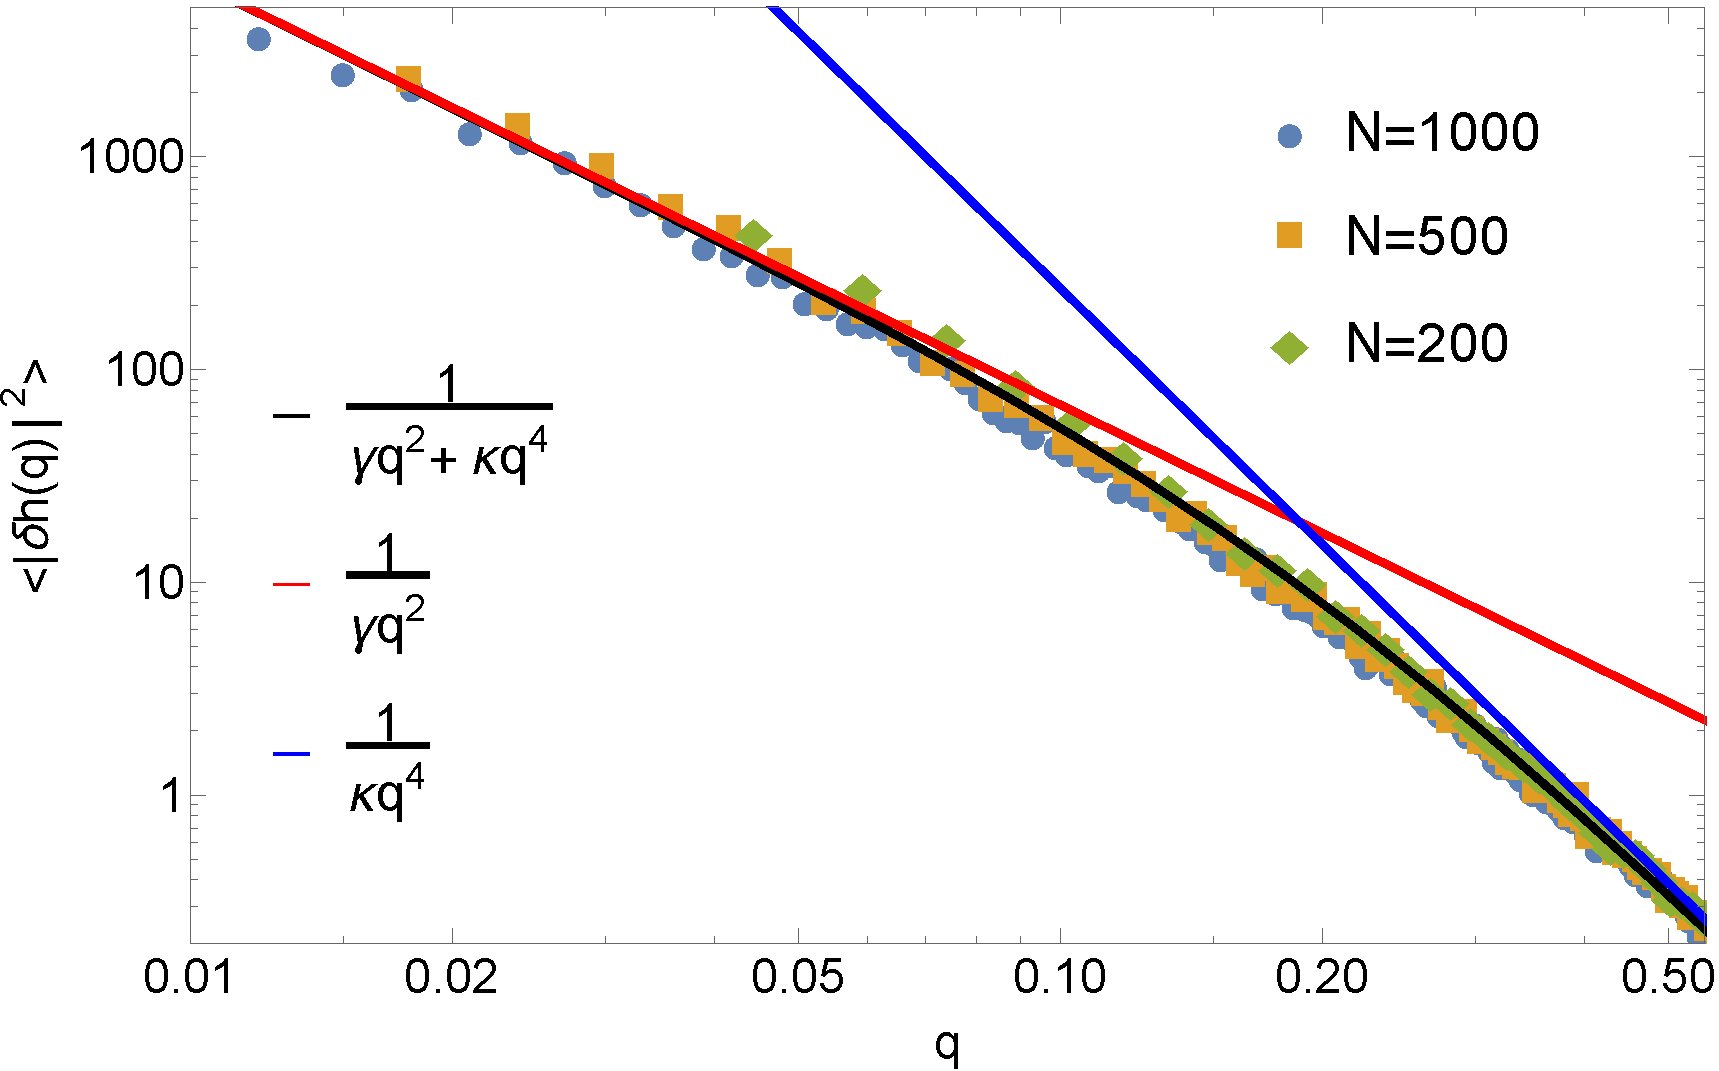
\includegraphics[scale=0.29]{Fig2.pdf}
\caption{Power spectrum of interfacial fluctuations at equilibrium. For small wavevectors, q, $|\delta h(q)|^2\propto q^{-2}$ while $|\delta h(q)|^2\propto q^{-4}$ at high q in agreement with expectations Eq.~\ref{eq:HelfrichFT}. The data here is for $k_s=4$ and $k_\theta = 6$. The diamond symbols are fluctuations of the assembly with 200 particles. The square symbols are fluctuations of the assembly with 500 particles. The circle symbols are fluctuation of the assembly with 1000 particles. Because the fluctuations here follow the Helfrich Hamiltonian, its standard deviation is exactly equal to its average magnitude due to the exponential nature of the distribution. Here $\gamma = 1.76$ and $\kappa =39.1$ from the fit} \label{fig:HelfrichScaling}
\end{figure}

\begin{figure}[tbb]
\centering
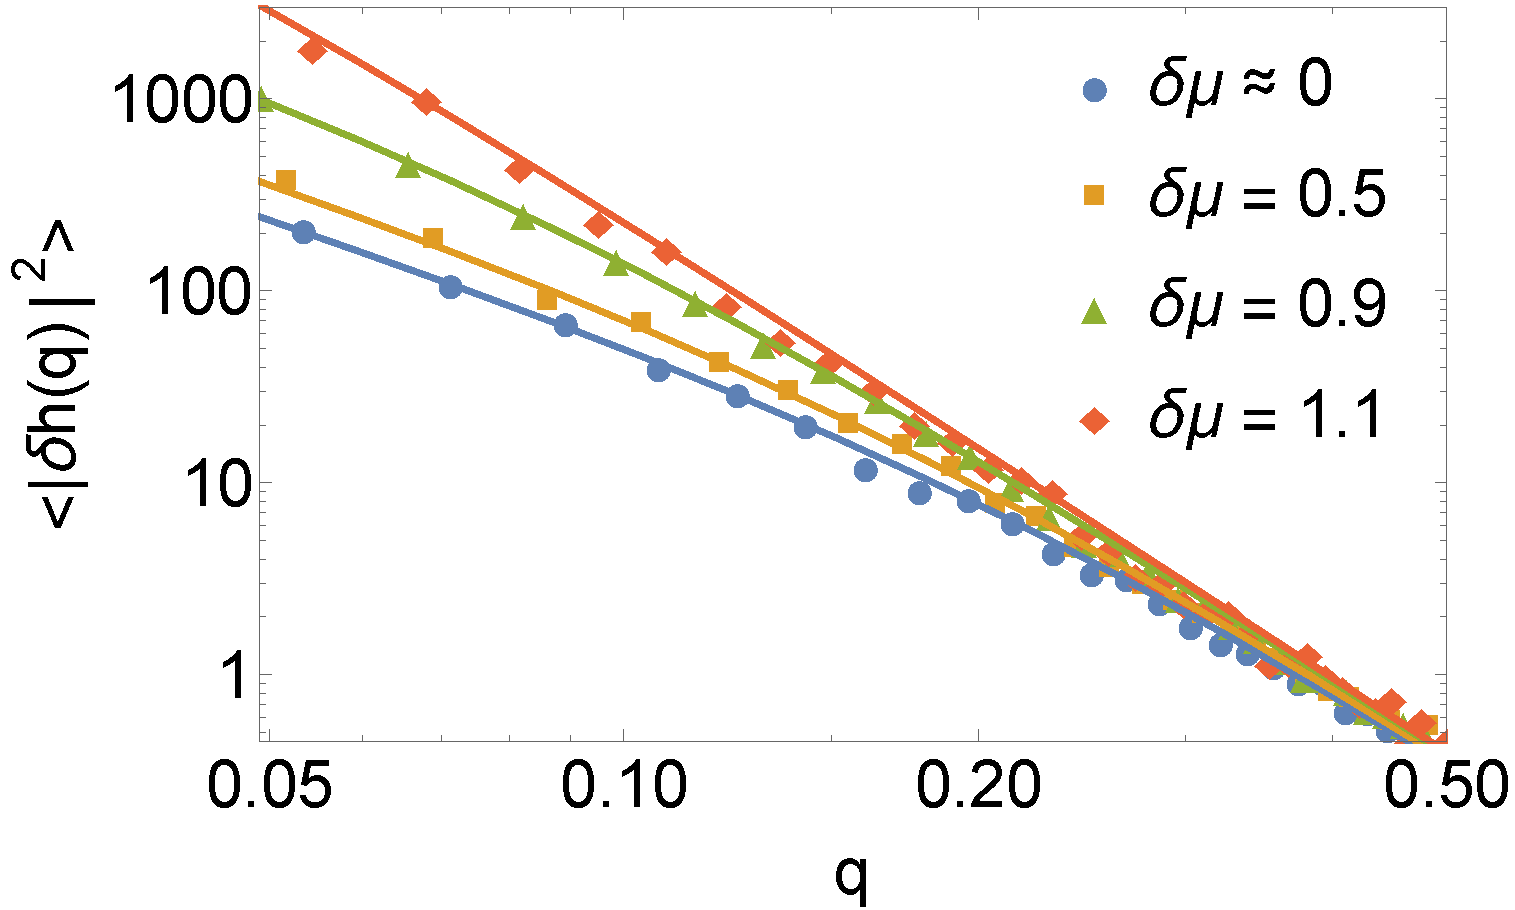
\includegraphics[scale=0.34]{Fig3.pdf}
\caption{Power spectrum of interfacial fluctuations at different $\delta\mu$. Fitting these curves to Eq.~\ref{eq:HelfrichFT} allows us to estimate $\gamma$ and $\kappa$ as described in the text. This analysis reveals that $\gamma_{\rm eff}$ decreases with increasing $\delta\mu$. The data here is for $k_s=4$ and $k_\theta = 6$.} \label{fig:Helfrich}
\end{figure}




\noindent{\it Simulations and results:} Our model consists system of particles in a ring like geometry interacting according to the Hamiltonian, 
\begin{equation}
\label{eq:Halmitonianl}
E=\sum_i^N{\frac{k_s}{2}(l_{i,i+1}-l_0)^2+k_\theta(\theta_i-\pi)^2}\,,
\end{equation}
where $l_{i,i+1}$ is the distance between particle $i$ and particle $i+1$, $l_0$ is the equilibrium distance and $\theta_i$ is the angle that particle $i$ makes with its neighbors. The growth dynamics of the Monte Carlo simulation are detailed in SI Fig S1. In short, in each Monte Carlo step, we attempt to add a particle from the bath or remove a random particle from the assembly with equal probability.   Events adding particles to the assembly are accepted with the probability $\rm{min}\{1,e^{(-\Delta E +\mu)/k_{\rm B} T}\}$ and events removing particles from the assembly are accepted with the probability $\rm{min}\{1,e^{(-\Delta E -\mu)/k_{\rm B} T}\}$. Here, the parameter $\mu$ can be regarded as the chemical potential of monomer units in the bath and $k_B T$ sets an energy scale. Unless specified otherwise, we set $k_{\rm B} T = 1$ for simplicity in the rest of the paper. 

The rate of growth of the elastic assembly can be tuned by varying the parameter $\mu$. Specifically, we find that there exists a \textit{coexistence} value of $\mu$, $\mu_{\rm coex}$, at which the assembly does not grow on average. The system is at equilibrium with its surroundings for this value of $\mu$. In the rest of the manuscript, we use the term equilibrium to refer to conditions where $\mu =\mu_{\rm coex}=\mu_{\rm eq}$, and the term non-equilibrium to refer to conditions where $\mu > \mu_{\rm eq}$. 

For values of $\mu$ above the coexistence value $\mu_{\rm eq}$, the system is driven away from equilibrium and the elastic ring polymer starts to grow. When $\delta\mu/k_{\rm B}T \equiv (\mu-\mu_{\rm eq})/k_{\rm B} T$ is small, the elastic assembly grows slowly and roughly retains its circular shape (see Movie: M1 in the SI). With increasing $\delta\mu/k_{\rm B} T$, the elastic assembly grows faster; its shape becomes more distorted (Movie: M2). Ultimately, the elastic assembly buckles resulting in spikes growing out of the circle as shown in Fig.~\ref{fig:phases} (Movie: M3). 

To study the above mentioned morphological changes (Fig.~\ref{fig:phases}), we examine how the fluctuations of the elastic ring polymer are modified as a function of its growth rate. Specifically, we divide the circumference of the assembly into $N$ equal segments with length $\langle l \rangle \equiv L/N$, where $N$ is the number of particles in the assembly at that instance of time and $L$ is the circumference of the assembly. 
 We then measure fluctuations in $\hat{h}(x_n)$ where $x_n\equiv n\langle l \rangle$, $\hat{h}(x_n)$ denotes the deviation of the $n^{\rm th}$ segment from the average radius of the elastic assembly, $\hat{h}(x_n)\equiv h(x_n) -\langle h \rangle$. The ensemble over which the fluctuations are measured was constructed by initiating simulations with a certain initial elastic assembly nucleus with size $N_0$ and allowing the nucleus to grow for a time $t_{\rm measure}$. In order to ensure that our results are not affected by choices of $N_0$ and $t_{\rm measure}$, simulations with multiple values of $N_0$ and $t_{\rm measure}$ were considered (See Fig.~\ref{fig:HelfrichScaling} and Fig. S7 and S8 in the SI~\cite{Supplementary}). In ensembles constructed in this manner, we measured $\langle |\delta h(q)|^2 \rangle$ where $\delta h(q)$ is the Fourier transform of the radial fluctuations defined with the convention: $\hat{h}(x_n)=\frac{1}{\sqrt{N}}\sum _q \delta h(q) \exp(iqx_n), q = \frac{2\pi m}{N\langle l \rangle}, m = 1, 2,...,N$. 

At or close to equilibrium, $\delta \mu /k_{\rm B} T \ll 1$, by measuring fluctuations and averaging over the above-described ensembles, we find that $\langle |\delta h(q)|^2 \rangle$ scales likes $q^{-2}$ in the low $q$ regime and scales like $q^{-4}$ in the high $q$ regime (Fig.~\ref{fig:HelfrichScaling}). This suggests that 
at equilibrium, the fluctuations of the elastic ring can be effectively described using the Helfrich Hamiltonian~\cite{W.Helfrich1973}:
\begin{equation}
E_{\rm eq}=\int \left \{\frac{\gamma_{\rm eq}}{2} (\nabla \hat{h})^2+  \frac{\kappa_{\rm eq}}{2} (\Delta \hat{h})^2\right \} dx.
\label{eq:Helfrich}
\end{equation}
Motivated by the scaling in Fig.~\ref{fig:HelfrichScaling}, we refer to the parameter $\gamma_{\rm eq}$ as an effective surface tension and the parameter $\kappa_{\rm eq}$ as an effective bending rigidity. We have tested the simulations with $k_s$ ranging from 2 to 4, and with $k_\theta$ ranging from 3 to 6. In these ranges, the fluctuations all follow the scaling of the Helfrich Hamiltonian. In addition, at equilibrium, $\gamma_{\rm eq}$ decreases with increasing $k_s$ and $k_{\theta}$. On the other hand, $\kappa_{\rm eq}$ seems to depend minimally on $k_s$ and decreases with decreasing $k_{\theta}$. We stress again that we are defining these elastic constants, $\gamma_{\rm eq}$ and $\kappa_{\rm eq}$ in the context of the ensembles defined above. 

Even as the assembly starts to grow, Fig.~\ref{fig:Helfrich} shows that the radial fluctuations are still described by an effective Helfrich Hamiltonian with renormalized surface tension and bending rigidity, $\gamma$ and $\kappa$ respectively. Indeed, Fig.~\ref{fig:Helfrich} shows that the average $\langle |\delta h(q)|^2 \rangle$ is well described by 
\begin{equation}
\langle |\delta h(q)|^2 \rangle \propto \frac{k_B T}{(\gamma q^2 + \kappa q^4)}\,,
\label{eq:HelfrichFT}
\end{equation}
in accordance with Eq.~\ref{eq:Helfrich} with renormalized effective surface tension and bending rigidity values. Closer inspection of the effective surface tension and bending rigidity extracted from Fig.~\ref{fig:Helfrich} shows that the effective surface tension,$\gamma$ decreases as $\delta \mu$ is increased, dropping to $\gamma\approx 0$ at a critical value of $\delta \mu=\delta \mu_c$ (Fig.~\ref{fig:HelfrichInstability}). Beyond this point, the elastic assembly buckles and undergoes a morphological transformation to ring populated by \textit{}{spikes}. The number of spikes appearing in a process increases with $\delta\mu$ and is proportional to the initial size of the assembly (see Fig.~\ref{fig:HelfrichInstability}) and remains constant during the growing period. 
Reflecting the diminished effective surface tension cost under non-equilibrium conditions, the configurations with spikes allow the system to grow with minimal penalties for stretching. The bending rigidity does not seem to change by a large amount as indicated by fits obtained from Fig.~\ref{fig:Helfrich} (see Fig.~S7 in the SI~\cite{Supplementary}). In order to study how these elastic quantities depend on membrane size, we extracted the effective renormalized values of the surface tension and bending rigidity for multiple values of initial size $N_0$ and simulation time $t_{\rm measure}$. We find that to a good numerical approximation, the effective elastic constants, $\gamma$, $\kappa$ and values of the parameters $\mu_{\rm coex}$, and $\delta \mu_c$, are time and size independent in all our simulations as shown in Fig.~\ref{fig:HelfrichScaling} (see Fig.~S7 and S8 in the SI~\cite{Supplementary}). 

%We again note that we performed numerical simulations with multiple initial sizes $N_0$ and multiple choices of $t_{\rm measure}$. The values of $\delta \mu$, $\gamma_{\rm eff}$. $\kappa_{\rm eff}$, $\delta \mu_c$ were independent of $N_0$ and $t_{\rm measure}$ in our numerical simulations. 

\begin{figure}[tbb]
\centering
\includegraphics[scale=0.25]{Fig4.pdf}
\caption{Phase diagram for data at $k_s=4$ and $k_\theta = 6$. As $\delta\mu$ is increased, the effective surface tension $\gamma$ decreases eventually reaching $\gamma\approx 0$ for $\delta\mu \approx 1.1$.  Increasing $\delta \mu$ beyond this value induces a morphological change to a configuration with spikes. The data was obtained with $N_0=200$. The red curve in the figure represents the surface tension $\gamma$ of the assembly before the instability. The error bar represents the 95\% confidence interval from fitting. After the instability, $\gamma$ is negative and cannot be measure using the Fourier transform technique. We then use the number of spikes (the blue curve) in the assembly, which can be used to infer the instabilities' wavelength, to indicate the systems at different drive post the instability. The blue curve in the figure represents the number of spikes} \label{fig:HelfrichInstability}
\end{figure}

\noindent{\it A non-equilibrium thermodynamic theory for renormalization of surface tension and morphological changes:} We now use ideas from stochastic thermodynamics to understand the trade-offs between non-equilibrium driving (as characterized by $\delta \mu$) and morphological changes in the structure of this elastic ring system (as characterized by the renormalized constants $\gamma$ and $\kappa$). A detailed molecular derivation is provided in the SI (see SI Sec: 6)~\cite{Supplementary}. Here, we provide a phenomenological derivation. We begin by noting that our numerical results suggest that even when the elastic ring is not at equilibrium, its fluctuations can be described in terms of an effective energy landscape, (Fig.~\ref{fig:Helfrich}). In this case, using the principles of stochastic thermodynamics, an expression for the entropy of the growing elastic system can effectively be written down as~\cite{Nguyen2016,Esposito2012}
\begin{equation}
\label{eq:entropysystem}
 TS=\left\langle N \right\rangle_t \frac{-F_{\rm{eff}} + \langle E_{\rm{eff}} \rangle _N}{N}\,,
\end{equation}
where $E_{\rm{eff}}$ is the effective elastic energy of a configuration in terms of the renormalized material parameters $\gamma$ and $\kappa$, $F_{\rm{eff}}$ is the Helmholtz free energy appropriate to $E_{\rm{eff}}$, $\langle...\rangle_N$ is the average of all microscopic configurations of the assembly at size $N\gg 1$ and $\langle N \rangle_t$ is the average size of the elastic ring after it has been allowed to grow for a time $t$. Since $d\langle N \rangle_t/dt > 0$ under non-equilibrium conditions $\delta\mu >0$, the entropy of the system changes as a function of time. 

We can similarly compute the change in the entropy of the bath as it supplies monomers to the elastic assembly and maintains constant chemical potential conditions. Specifically, in the limit that the bath size is much larger than the size of any elastic assembly, the change in entropy of the bath after a time t, $\Delta S_{\rm bath}$, can be written as :
\begin{equation}
\label{eq:entropybath}
 T\Delta S_{\rm bath}=-\left\langle N \right\rangle_t \frac{-F_{\rm{eq}} + \langle E_{\rm{eq}} \rangle _N-N\delta\mu}{N}
\end{equation}
By combining Eq.~\ref{eq:entropysystem} and Eq.~\ref{eq:entropybath}, we can write down the total entropy of the process, which must be nonnegative according to the second law of thermodynamics~\cite{Esposito2012}:
\begin{equation}
\begin{split}
\label{eq:entropytotal}
\frac{dS_{\rm total}}{dt}&=\frac{dS}{dt} +\frac{dS_{\rm bath}}{dt}\\
&= \frac{d\langle N\rangle}{dt}\left ( \delta\mu-\langle\epsilon_{\rm diss}\rangle \right) \geq 0
\end{split}
\end{equation}
Here $\langle\epsilon_{\rm diss}\rangle=\left (\left\langle E_{\rm eq}-E_{\rm{eff}}\right\rangle _N-\left ( F_{\rm eq}-F_{\rm{eff}}\right )\right )/N$. $\langle\epsilon_{\rm diss}\rangle$ can be thought as the minimum work required to transform the energy landscape of the system from $E_{\rm eq}$ to $E_{\rm eff}$ using a driving force. The driving force here can come from many sources such as chemical activity and mechanical work. In this letter, the driving force here is the extra chemical potential we put into the bath.  For a growing system, $\frac{d\langle N \rangle}{dt}$ is positive thus reducing Eq.~\ref{eq:entropytotal} to:
\begin{equation}
\label{eq:firstbound}
\delta\mu-\langle\epsilon_{\rm diss}\rangle\geq0
\end{equation}

Tighter, and more informative bounds can be obtained by using the recently derived uncertainty relations that relate the entropy production to the fluctuations of various fluxes in the system~\cite{Barato2015, Gingrich2016,Nguyen2016}. For our purposes, we consider the fluctuations in the growth rate flux, $\dot{N}$. An application of the thermodynamic uncertainty relations then implies the following tighter bound: 
\begin{equation}
\label{eq:secondbound}
\delta\mu-\langle\epsilon_{\rm diss}\rangle\geq\frac{v k_{\rm B} T}{D}\, 
\end{equation}
where $v=\frac{d\langle N\rangle}{dt}$ is the growth rate of the assembly, and $D=\lim_{\tau\to\infty}\frac{\langle\Delta N^2\rangle}{2\tau}$  is the diffusion constant of the size fluctuations of the assembly. The equality in Eq.~\ref{eq:secondbound} is achieved in the linear response limit. 

The bounds in Eq.~\ref{eq:firstbound} and Eq.~\ref{eq:secondbound} constrain the allowed values of $\gamma$ and $\kappa$ given $\delta \mu$, the equilibrium elastic constants $\gamma_{\rm eq}, \kappa_{\rm eq}$ and the ratio $vk_{\rm B}T/D$. The non-equilibrium driving due to $\delta \mu$ can be used to maintain a growth rate and simultaneously renormalize fluctuations in the growing assembly. Eq.~\ref{eq:secondbound} assigns a thermodynamic cost for maintaining a growth rate, $v/D$, and a thermodynamic cost for renormalizing fluctuations, $\langle \epsilon_{\rm diss}\rangle$, and requires that net driving force, $\delta \mu$, be greater than the sum of the aforementioned thermodynamic costs. 

Note that Eqs.~\ref{eq:firstbound},~\ref{eq:secondbound} are minimally dependent on the kinetics of the growth process. A detailed microscopic proof of Eq.~\ref{eq:firstbound}, Eq.~\ref{eq:secondbound} is provided in the SI Sec 6~\cite{Supplementary}. This detailed microscopic proof does not require the membrane system to be constrained to two dimensions and can be readily applied to three dimensional membranes. Hence, we anticipate that the bounds in Eq.~\ref{eq:firstbound} and Eq.~\ref{eq:secondbound} can be applied to a broader class of non-equilibrium membrane growth processes (see SI Sec 6~\cite{Supplementary}). Finally we note that both the phenomenological derivation provided above and the detailed derivation provided in the SI assume that the fluctuations in the growth rate are minimally correlated with fluctuations in the configurations. As explained in the SI, formally this amounts to a mean field assumption that the growth rate of a particular configuration is simply proportional to the probability with which it is generated in the steady state. Extensions of Eqs.~\ref{eq:firstbound},~\ref{eq:secondbound} to non-mean field regimes are provided in the SI. Supported by numerical results detailed below, we note that the mean field assumption for growth rate statistics seems to work well for our membrane systems. In practice the mean field assumption can be shown to be exact for a class of lattice based non-equilibrium growth models~\cite{Nguyen2016}. 

\begin{figure}[tbb]
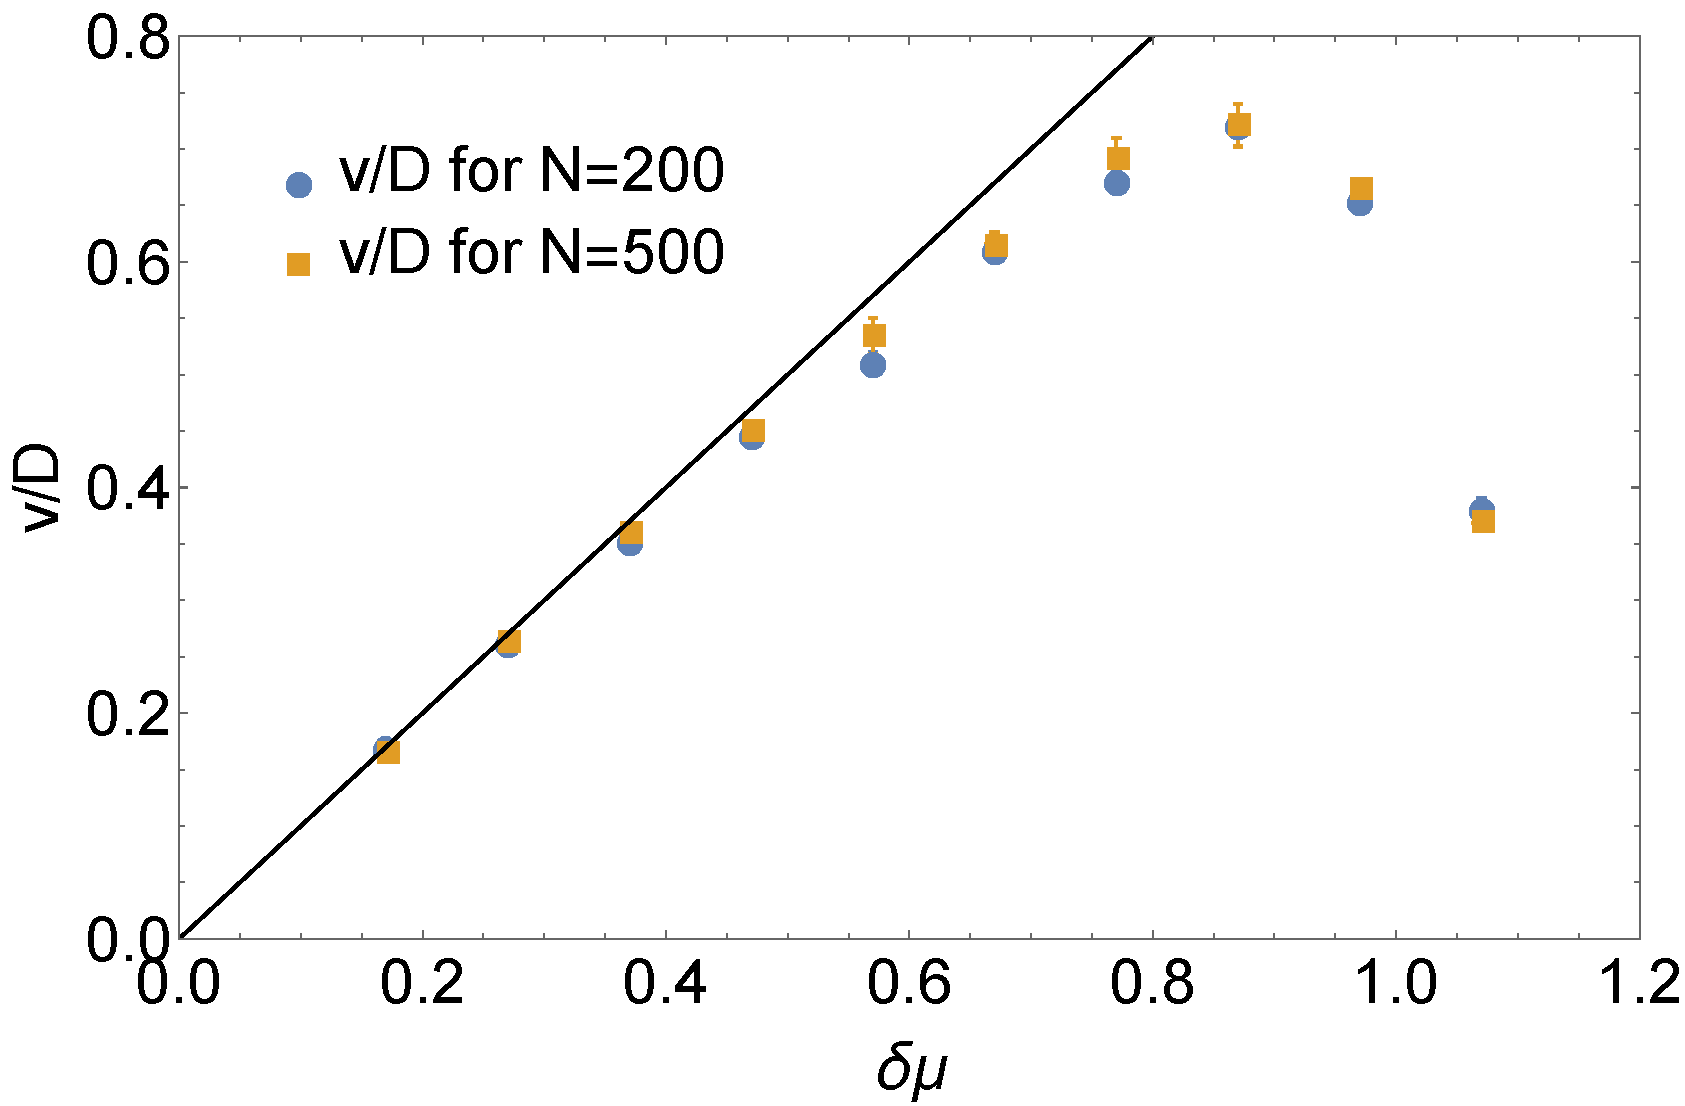
\includegraphics[scale=0.3]{Fig5.pdf}
\caption{$\frac{v}{D}$ vs. $\delta\mu$. In this case, $k_{\rm B}T$ is set to 1. The dark line is predicted from linear response. The error bar represents the 95\% confidence interval from the fit $\delta\mu=v/D$. The blue dot is from the assemblies of 200 particles, while the orange dot is from the assemblies of 500 particles. The two measurements overlaps with some minor error.}
\label{fig:LinearResponse}
\end{figure}

Before proceeding to use Eq.~\ref{eq:secondbound} to elucidate how the thermodynamic driving forces control the renormalization of material properties and morphologies, we first consider Eq.~\ref{eq:secondbound} without the term non-negative term $\langle \epsilon_{\rm{diss}}\rangle$~\footnote{The statement $\langle\epsilon_{\rm diss}\rangle\geq 0$ can be proven by applying Jensen's inequality to: $\langle\exp\left[-(E_{\rm{eq}}-E_{\rm{eff}})\right]\rangle_N=\exp\left[-(G_{\rm{eq}}-G_{\rm{eff}})\right]$}. The bound in Eq.~\ref{eq:secondbound} reduces to the following relation between driving force $\delta \mu$ and ratio $v/D$, $\delta\mu\geq\frac{v k_B T}{D}$. In Fig.~\ref{fig:LinearResponse} we numerically verify that our simulations at two different sizes do indeed satisfy this simplified connection. Further, in the limit of slow driving, $\delta \mu/k_B T\ll 1$, Fig.~\ref{fig:LinearResponse} reveals that most of the driving force is used up in maintaining a growth rate with very little remaining for renormalization of material parameters. In this limit, $\delta \mu \approx v/D$. 
At larger values of the driving, $\delta \mu$ deviates significantly from $v/D$. Larger value of the thermodynamic cost associated with renormalized fluctuations, $\langle \epsilon_{\rm diss}\rangle$, are hence allowed by our thermodynamic bound in these regimes. Indeed, our simulations (Fig.~\ref{fig:phases}) show how a dramatic change in morphologies can be achieved for $\delta \mu/k_B T \approx 1$. 

We will now use Eq.~\ref{eq:secondbound} to understand how $\gamma$ can be controlled by tuning $\delta \mu$. As first approximation, given the relatively slow renormalization of the bending rigidity, we will set $\kappa=\kappa_{\rm eq}$ (see Fig S7 in SI). Within this approximation (see SI Sec 7~\cite{Supplementary}), we obtain the following simplified expression for $\langle \epsilon_{\rm diss} \rangle$: 
\begin{equation}
\label{eq:epsilonexpress}
 \langle\epsilon_{\rm diss}\rangle =\frac{k_{\rm B}T\lambda}{4\pi}\left ( \frac{(\gamma + \gamma_{\rm eq})\phi-2\sqrt{\gamma\gamma_{\rm eq}}\phi^*}{\sqrt{\gamma \kappa_{\rm eq}}}-\frac{2\pi \xi}{\lambda} \right)
\end{equation}
Here $\phi=\arctan(\frac{2\pi\sqrt{\kappa_{\rm eq}}}{\lambda\sqrt{\gamma}}), \phi^*=\arctan(\frac{2\pi\sqrt{\kappa_{\rm eq}}}{\lambda\sqrt{\gamma_{\rm{eq}}}})$, $\xi=\ln(\frac{\gamma_{\rm{eq}}\lambda^2+4\pi^2\kappa_{\rm eq}}{\gamma\lambda^2+4\pi^2\kappa_{\rm eq}})$, and $\lambda$ is the smallest wavelength allowed by the assembly which we will take to be $l_0$. Using this expression for $\epsilon_{\rm diss}$, Eq.~\ref{eq:firstbound} and Eq.~\ref{eq:secondbound} can be used to predict bounds on how $\gamma$ changes with the non-equilibrium driving $\delta \mu$. These predictions are plotted in Fig.~\ref{fig:PhaseDiagram} alongside the scaling of $\gamma$ with $\delta \mu$ extracted from simulations. 

\begin{figure}[tbb]
\centering
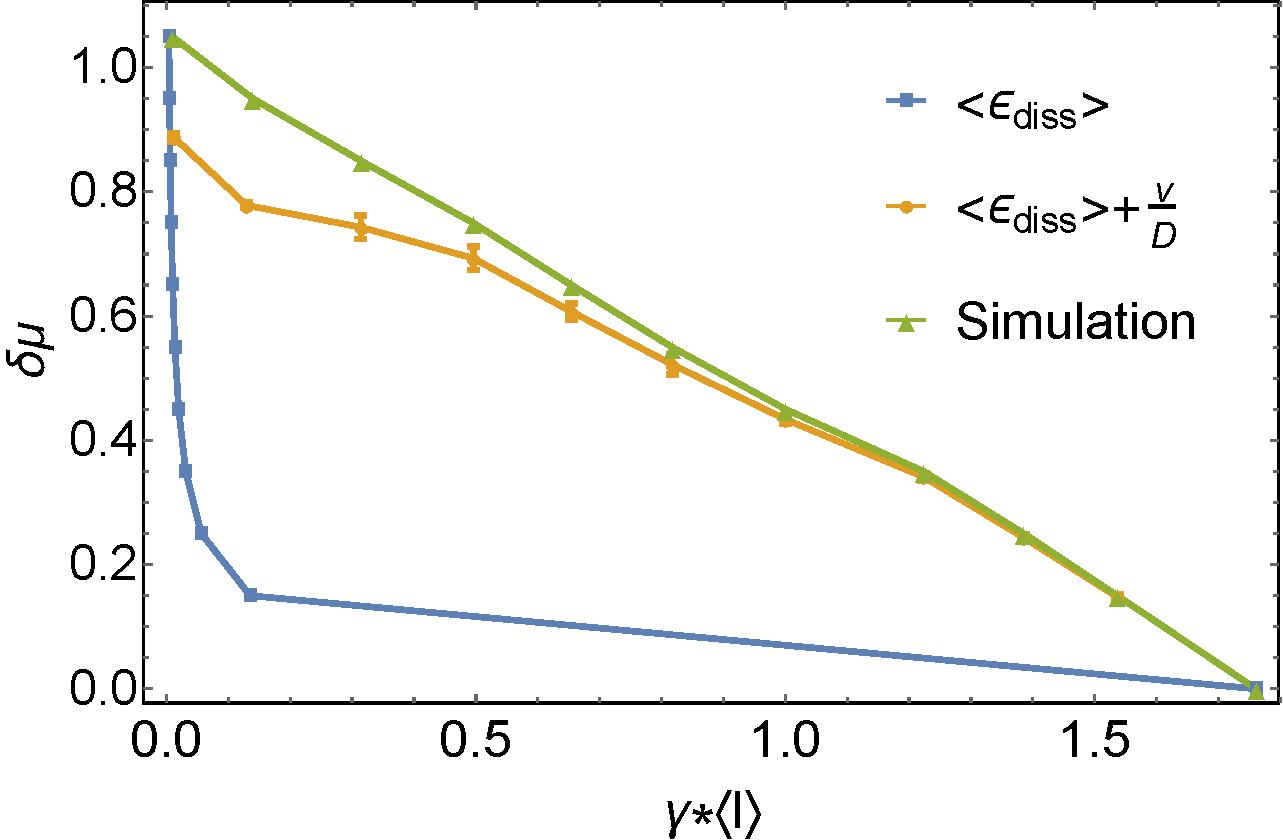
\includegraphics[scale=0.38]{Fig6.pdf}
\caption{Thermodynamic bounds on the surface tension as a function of the non-equilibrium driving force $\delta\mu$. The bound stipulated by the blue curve is from Eq.~\ref{eq:firstbound}. The bound stipulated by the orange curve is from Eq.~\ref{eq:secondbound}. The green curve is obtained by measuring $\gamma$ from simulations and is consistent with the bounds specified by Eq.~\ref{eq:firstbound} and Eq.~\ref{eq:secondbound}. These bounds provide rough estimates for the energetic costs required to modify the morphology and fluctuations in the elastic membrane. The error bars in the second bound is obtained from $95\%$ confidence intervals of fitting $\frac{v}{D}$.}\label{fig:PhaseDiagram}
\end{figure}

Fig.~\ref{fig:PhaseDiagram} shows how ideas from stochastic thermodynamics can be used to predict how material properties such as the surface tension can be modified in the presence of non-equilibrium forces. In particular, the lower bound suggested by Eq.~\ref{eq:secondbound} is surpisingly close to the actual non-equilibrium driving force $\delta \mu$ required to renormalize membrane tension and induce morphological transformations ($\gamma\sim 0$). Unlike the usual approaches, the bounds here do not require extensive knowledge of the kinetics of the system. Indeed, as evidenced by the performance of the bound in Eq.~\ref{eq:secondbound} in Fig.~\ref{fig:PhaseDiagram}, our results show how a large component of the non-equilibrium renormalization of membrane material properties is effectively controlled by two (experimentally accessible) parameters, the driving force $\delta \mu$, and the ratio $v/D$. 

%$\delta \mu$, and the ratio $v/D$, are sufficient to capture most of the non-equilibrium renormalization of membrane material properties. 

%Instead, for these bounds, one needs to identify relevant parameter combinations (in this case $\gamma$ and $v/D$) that capture most of the non-equilibrium changes. 


%As expected from linear response theory, the bound in Eq.~\ref{eq:secondbound} agrees very well with simulation results close to equilibrium. \textbf{ Away from equilibrium, Eq.~\ref{eq:secondbound} indeed provides a lower bound for $\delta \mu$. As we go very far from equilibrium and approach the instability $\gamma_{\rm eff}\approx 0$, where linear response should fail (see Fig.~\ref{fig:LinearResponse}), our bounds still hold and can give a quantitative predictions on the point of instability. Fig.~\ref{fig:PhaseDiagram} shows how ideas from stochastic thermodynamics can be used to predict how material properties such as the surface tension, can be modified in the presence of non-equilibrium forces.} It also provides a thermodynamic lower bound for the minimum non-equilibrium driving force $\delta \mu$ required to obtain $\gamma_{\rm eff}\sim 0$ and induce morphological transformations in the system. Unlike the usual approach, the bounds here do not require extensive knowledge of the kinetics of the system. Instead, for these bounds, one need to identify relevant parameter combinations (in this case $\gamma$ and $v/D$) that capture most of the non-equilibrium changes. 


The role played by non-equilibrium forces in biological processes such as those responsible for modulating cell shapes and dynamics is well established~\cite{McMahon2005,Stachowiak2012,Chen2016,Turlier2016,Rao2001,Solon2006}. In this paper we have shown how ideas from stochastic thermodynamics, in particular an adaptation of the recently derived thermodynamic uncertainty relations, can be used to obtain general non-equilibrium thermodynamic constraints on membrane morphologies and material properties. Our thermodynamic bounds are minimal dependent on the details of the kinetic processes responsible for membrane growth. We anticipate that such thermodynamic ideas will find broad applicability and reveal how material properties and morphologies can be robustly controlled even far from equilibrium. 

%we have probed the tradeoffs between energy consumption and organization in a model non-equilibrium membrane growth process. Although in this letter, the driving force of our system is an extra chemical potential, $\delta\mu$, we anticipate that the prescription we provided here can be extended to include other sources of non-equilibrium activity. Hence, given the minimal kinetic detail required by our effectively thermodynamic bounds, we expect that our results will find broad applicability in more complex varieties of membrane reorganization processes in synthetic~\cite{Zwicker2017} and biological systems. 

%The validity of the above argument lies on the assumption that an entropy production term can be constructed for such process. In addition, we have also assume that the system can be described using an effective Helfrich Hamiltonian and this simply might not be the case. For the second part, we want to stress that at this time, we have only used very little information on the system: only the means amplitude of the mode which is zero and their variance. Without more information on the system, it would not be optimal to attempt the above approach with more complicated distribution. As for the first part, in general, in order to derive an expression for the entropy production of the process, one has to construct an Markov model with master equation or an Stochastic Differential Equation which by no mean a trivial task. Here, by using the approach that we previously developed, we are able to write out an expression for the entropy production with minimal information. However, to further illustrate that it is possible to describe our system with an entropy production, we have constructed a Markov model that can describe our system qualitatively and derived an entropy production term from it. 
%\begin{figure}[tbb]
%\centering
%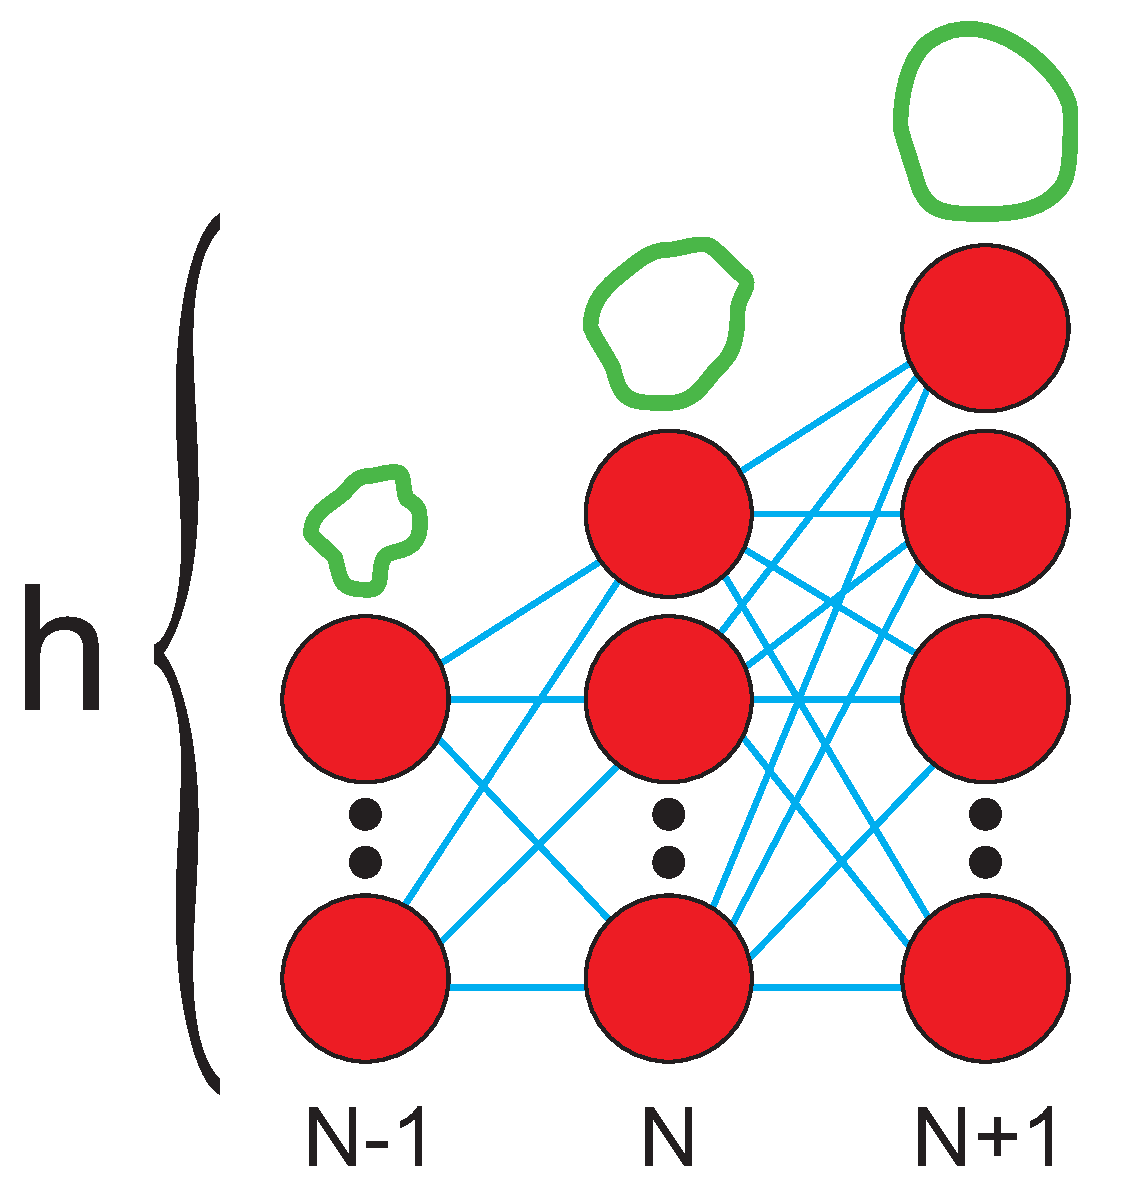
\includegraphics[scale=0.33]{markovmodelparticleinaringver2.pdf}
%\caption{Schematic of our Markov network. The vertical rungs represents the amplitude of our modes while the horizontal line represents the number of particle. The number of nodes here are just for illustration and does not reflect the actual number of nodes that increase with system size} \label{fig:markov}
%\end{figure}

%In our model, working in Fourier space, we imagine a Markov network with nodes describing the fluctuation of $\delta h(q)$ of the system (Fig 8). The vertical rungs will indicate the amplitude of the modes while the horizontal line describe the system size. Because the number of modes is proportional to the number of particles, the number of nodes our Markov model can access also increases with the assembly size. In fact, the state space accessible by our model scales like $\mathbb{R}^N$. Adding a particle is like introducing a small wavelength mode to the assembly in which the amplitude, $|h|^2$ , is chosen according to $P\propto  \textrm{Exp}[-\Sigma\kappa q^4 |h|^2]$. The acceptance rate of such configuration is $\mathit{Min}[ \textrm{Exp}[(-\Sigma\gamma q^2 |h|^2+N\mu)],1]$. We then look at the steady state mode probability distribution of the assembly and attempt to remove it with accepting rate: $\mathit{Min}[\textrm{Exp}[(\Sigma\gamma q^2 |h|^2-N\mu)],1]$.  Because the modes of the system keep increasing with the assembly size, the transition rate of our Markov model also depends on time. Specifically, for each new mode, we have to add an extra term $-\gamma q^2 |h|^2+\mu$ to the addition acceptation rate and $\gamma q^2 |h|^2-\mu$ to the removal acceptance rate. Since we only care about the steady state of the process, we can approximate our Markov process with a Poisson Process \cite{Maes2008} with an effective arrival rate $\lambda$ which like the acceptance rates of the Markov process has to increase with $N$ as well. The probability at certain time, t, for the arrival of a particle of a Poisson process is: $\lambda t \textrm{Exp}(-\lambda t)$. Thus, if one cannot increase the rate $\lambda$, the time has to increase to compensate for the effect of adding more modes into the system.  In order words, when the assembly only has 1 particle and it would take only certain time $t$ to add a particle. For a system with N particle, one would require $Nt$. This is reflected in the square root growth rate of our simulations.  With a few line of algebra, it can be shown that the steady state distribution of this model is only in Gaussian form when it is at equilibrium and at very far from it.  In addition, this model cannot give an instability. However, it does give the same scaling of $|h^2|$ as our simulations that is as one increase $\delta\mu$, the surface tension $\gamma$ will decrease.
The authors acknowledge support from NSF DMR-
MRSEC  1420709, NSF GFRP and the  University  of  Chicago
 
%\bibliography{References02232018}
%merlin.mbs apsrev4-1.bst 2010-07-25 4.21a (PWD, AO, DPC) hacked
%Control: key (0)
%Control: author (72) initials jnrlst
%Control: editor formatted (1) identically to author
%Control: production of article title (-1) disabled
%Control: page (0) single
%Control: year (1) truncated
%Control: production of eprint (0) enabled
\begin{thebibliography}{36}%
\makeatletter
\providecommand \@ifxundefined [1]{%
 \@ifx{#1\undefined}
}%
\providecommand \@ifnum [1]{%
 \ifnum #1\expandafter \@firstoftwo
 \else \expandafter \@secondoftwo
 \fi
}%
\providecommand \@ifx [1]{%
 \ifx #1\expandafter \@firstoftwo
 \else \expandafter \@secondoftwo
 \fi
}%
\providecommand \natexlab [1]{#1}%
\providecommand \enquote  [1]{``#1''}%
\providecommand \bibnamefont  [1]{#1}%
\providecommand \bibfnamefont [1]{#1}%
\providecommand \citenamefont [1]{#1}%
\providecommand \href@noop [0]{\@secondoftwo}%
\providecommand \href [0]{\begingroup \@sanitize@url \@href}%
\providecommand \@href[1]{\@@startlink{#1}\@@href}%
\providecommand \@@href[1]{\endgroup#1\@@endlink}%
\providecommand \@sanitize@url [0]{\catcode `\\12\catcode `\$12\catcode
  `\&12\catcode `\#12\catcode `\^12\catcode `\_12\catcode `\%12\relax}%
\providecommand \@@startlink[1]{}%
\providecommand \@@endlink[0]{}%
\providecommand \url  [0]{\begingroup\@sanitize@url \@url }%
\providecommand \@url [1]{\endgroup\@href {#1}{\urlprefix }}%
\providecommand \urlprefix  [0]{URL }%
\providecommand \Eprint [0]{\href }%
\providecommand \doibase [0]{http://dx.doi.org/}%
\providecommand \selectlanguage [0]{\@gobble}%
\providecommand \bibinfo  [0]{\@secondoftwo}%
\providecommand \bibfield  [0]{\@secondoftwo}%
\providecommand \translation [1]{[#1]}%
\providecommand \BibitemOpen [0]{}%
\providecommand \bibitemStop [0]{}%
\providecommand \bibitemNoStop [0]{.\EOS\space}%
\providecommand \EOS [0]{\spacefactor3000\relax}%
\providecommand \BibitemShut  [1]{\csname bibitem#1\endcsname}%
\let\auto@bib@innerbib\@empty
%</preamble>
\bibitem [{\citenamefont {Battle}\ \emph {et~al.}(2016)\citenamefont {Battle},
  \citenamefont {Broedersz}, \citenamefont {Fakhri}, \citenamefont {Geyer},
  \citenamefont {Howard}, \citenamefont {Schmidt},\ and\ \citenamefont
  {MacKintosh}}]{Battle604}%
  \BibitemOpen
  \bibfield  {author} {\bibinfo {author} {\bibfnamefont {C.}~\bibnamefont
  {Battle}}, \bibinfo {author} {\bibfnamefont {C.~P.}\ \bibnamefont
  {Broedersz}}, \bibinfo {author} {\bibfnamefont {N.}~\bibnamefont {Fakhri}},
  \bibinfo {author} {\bibfnamefont {V.~F.}\ \bibnamefont {Geyer}}, \bibinfo
  {author} {\bibfnamefont {J.}~\bibnamefont {Howard}}, \bibinfo {author}
  {\bibfnamefont {C.~F.}\ \bibnamefont {Schmidt}}, \ and\ \bibinfo {author}
  {\bibfnamefont {F.~C.}\ \bibnamefont {MacKintosh}},\ }\href {\doibase
  10.1126/science.aac8167} {\bibfield  {journal} {\bibinfo  {journal}
  {Science}\ }\textbf {\bibinfo {volume} {352}},\ \bibinfo {pages} {604}
  (\bibinfo {year} {2016})}\BibitemShut {NoStop}%
\bibitem [{\citenamefont {Lan}\ \emph {et~al.}(2012)\citenamefont {Lan},
  \citenamefont {Sartori}, \citenamefont {Neumann}, \citenamefont {Sourjik},\
  and\ \citenamefont {Tu}}]{Lan2012}%
  \BibitemOpen
  \bibfield  {author} {\bibinfo {author} {\bibfnamefont {G.}~\bibnamefont
  {Lan}}, \bibinfo {author} {\bibfnamefont {P.}~\bibnamefont {Sartori}},
  \bibinfo {author} {\bibfnamefont {S.}~\bibnamefont {Neumann}}, \bibinfo
  {author} {\bibfnamefont {V.}~\bibnamefont {Sourjik}}, \ and\ \bibinfo
  {author} {\bibfnamefont {Y.}~\bibnamefont {Tu}},\ }\href {\doibase
  10.1038/nphys2276} {\bibfield  {journal} {\bibinfo  {journal} {Nature
  physics}\ }\textbf {\bibinfo {volume} {8}},\ \bibinfo {pages} {422} (\bibinfo
  {year} {2012})}\BibitemShut {NoStop}%
\bibitem [{\citenamefont {Mehta}\ and\ \citenamefont
  {Schwab}(2012)}]{Mehta2012}%
  \BibitemOpen
  \bibfield  {author} {\bibinfo {author} {\bibfnamefont {P.}~\bibnamefont
  {Mehta}}\ and\ \bibinfo {author} {\bibfnamefont {D.~J.}\ \bibnamefont
  {Schwab}},\ }\href {\doibase 10.1073/pnas.1207814109} {\bibfield  {journal}
  {\bibinfo  {journal} {Proceedings of the National Academy of Sciences}\
  }\textbf {\bibinfo {volume} {109}},\ \bibinfo {pages} {17978} (\bibinfo
  {year} {2012})}\BibitemShut {NoStop}%
\bibitem [{\citenamefont {Whitelam}\ \emph {et~al.}(2014)\citenamefont
  {Whitelam}, \citenamefont {Hedges},\ and\ \citenamefont
  {Schmit}}]{Whitelam2014}%
  \BibitemOpen
  \bibfield  {author} {\bibinfo {author} {\bibfnamefont {S.}~\bibnamefont
  {Whitelam}}, \bibinfo {author} {\bibfnamefont {L.~O.}\ \bibnamefont
  {Hedges}}, \ and\ \bibinfo {author} {\bibfnamefont {J.~D.}\ \bibnamefont
  {Schmit}},\ }\href {\doibase 10.1103/PhysRevLett.112.155504} {\bibfield
  {journal} {\bibinfo  {journal} {Physical Review Letter}\ }\textbf {\bibinfo
  {volume} {112}},\ \bibinfo {pages} {155504} (\bibinfo {year}
  {2014})}\BibitemShut {NoStop}%
\bibitem [{\citenamefont {Hopfield}(1974)}]{Hopfield1974}%
  \BibitemOpen
  \bibfield  {author} {\bibinfo {author} {\bibfnamefont {J.~J.}\ \bibnamefont
  {Hopfield}},\ }\href {http://www.pnas.org/content/71/10/4135.abstract}
  {\bibfield  {journal} {\bibinfo  {journal} {Proceedings of the National
  Academy of Sciences}\ }\textbf {\bibinfo {volume} {71}},\ \bibinfo {pages}
  {4135} (\bibinfo {year} {1974})}\BibitemShut {NoStop}%
\bibitem [{\citenamefont {Murugan}\ \emph {et~al.}(2012)\citenamefont
  {Murugan}, \citenamefont {Huse},\ and\ \citenamefont
  {Leibler}}]{Murugan2012}%
  \BibitemOpen
  \bibfield  {author} {\bibinfo {author} {\bibfnamefont {A.}~\bibnamefont
  {Murugan}}, \bibinfo {author} {\bibfnamefont {D.~A.}\ \bibnamefont {Huse}}, \
  and\ \bibinfo {author} {\bibfnamefont {S.}~\bibnamefont {Leibler}},\
  }\href@noop {} {\bibfield  {journal} {\bibinfo  {journal} {Proceedings of the
  National Academy of Sciences}\ }\textbf {\bibinfo {volume} {109}},\ \bibinfo
  {pages} {12034} (\bibinfo {year} {2012})}\BibitemShut {NoStop}%
\bibitem [{\citenamefont {Murugan}\ and\ \citenamefont
  {Vaikuntanathan}(2016)}]{Murugan2016}%
  \BibitemOpen
  \bibfield  {author} {\bibinfo {author} {\bibfnamefont {A.}~\bibnamefont
  {Murugan}}\ and\ \bibinfo {author} {\bibfnamefont {S.}~\bibnamefont
  {Vaikuntanathan}},\ }\href {\doibase 10.1007/s10955-015-1445-0} {\bibfield
  {journal} {\bibinfo  {journal} {Journal of Statistical Physics}\ }\textbf
  {\bibinfo {volume} {162}},\ \bibinfo {pages} {1183} (\bibinfo {year}
  {2016})}\BibitemShut {NoStop}%
\bibitem [{\citenamefont {Murugan}\ and\ \citenamefont
  {Vaikuntanathan}(2017)}]{Vaikunt2017}%
  \BibitemOpen
  \bibfield  {author} {\bibinfo {author} {\bibfnamefont {A.}~\bibnamefont
  {Murugan}}\ and\ \bibinfo {author} {\bibfnamefont {S.}~\bibnamefont
  {Vaikuntanathan}},\ }\href {\doibase http://dx.doi.org/10.1038/ncomms13881}
  {\bibfield  {journal} {\bibinfo  {journal} {Nature Communications}\ }\textbf
  {\bibinfo {volume} {8}},\ \bibinfo {pages} {13881} (\bibinfo {year}
  {2017})}\BibitemShut {NoStop}%
\bibitem [{\citenamefont {Barato}\ and\ \citenamefont
  {Seifert}(2017)}]{Barato2017}%
  \BibitemOpen
  \bibfield  {author} {\bibinfo {author} {\bibfnamefont {A.~C.}\ \bibnamefont
  {Barato}}\ and\ \bibinfo {author} {\bibfnamefont {U.}~\bibnamefont
  {Seifert}},\ }\href {\doibase 10.1103/PhysRevE.95.062409} {\bibfield
  {journal} {\bibinfo  {journal} {Physical Review E}\ }\textbf {\bibinfo
  {volume} {95}},\ \bibinfo {pages} {062409} (\bibinfo {year}
  {2017})}\BibitemShut {NoStop}%
\bibitem [{\citenamefont {McMahon}\ and\ \citenamefont
  {Gallop}(2005)}]{McMahon2005}%
  \BibitemOpen
  \bibfield  {author} {\bibinfo {author} {\bibfnamefont {H.~T.}\ \bibnamefont
  {McMahon}}\ and\ \bibinfo {author} {\bibfnamefont {J.~L.}\ \bibnamefont
  {Gallop}},\ }\href {\doibase 10.1038/nature04396} {\bibfield  {journal}
  {\bibinfo  {journal} {Nature}\ }\textbf {\bibinfo {volume} {438}},\ \bibinfo
  {pages} {590} (\bibinfo {year} {2005})}\BibitemShut {NoStop}%
\bibitem [{\citenamefont {Turlier}\ \emph {et~al.}(2016)\citenamefont
  {Turlier}, \citenamefont {Fedosov}, \citenamefont {Audoly}, \citenamefont
  {Auth}, \citenamefont {Gov}, \citenamefont {Sykes}, \citenamefont {Joanny},
  \citenamefont {Gompper},\ and\ \citenamefont {Betz}}]{Turlier2016}%
  \BibitemOpen
  \bibfield  {author} {\bibinfo {author} {\bibfnamefont {H.}~\bibnamefont
  {Turlier}}, \bibinfo {author} {\bibfnamefont {D.~A.}\ \bibnamefont
  {Fedosov}}, \bibinfo {author} {\bibfnamefont {B.}~\bibnamefont {Audoly}},
  \bibinfo {author} {\bibfnamefont {T.}~\bibnamefont {Auth}}, \bibinfo {author}
  {\bibfnamefont {N.~S.}\ \bibnamefont {Gov}}, \bibinfo {author} {\bibfnamefont
  {C.}~\bibnamefont {Sykes}}, \bibinfo {author} {\bibfnamefont {J.~F.}\
  \bibnamefont {Joanny}}, \bibinfo {author} {\bibfnamefont {G.}~\bibnamefont
  {Gompper}}, \ and\ \bibinfo {author} {\bibfnamefont {T.}~\bibnamefont
  {Betz}},\ }\href {\doibase 10.1038/nphys3621} {\bibfield  {journal} {\bibinfo
   {journal} {Nature Physics}\ }\textbf {\bibinfo {volume} {12}},\ \bibinfo
  {pages} {513} (\bibinfo {year} {2016})}\BibitemShut {NoStop}%
\bibitem [{\citenamefont {Stachowiak}\ \emph {et~al.}(2012)\citenamefont
  {Stachowiak}, \citenamefont {Schmid}, \citenamefont {Ryan}, \citenamefont
  {Ann}, \citenamefont {Sasaki}, \citenamefont {Sherman}, \citenamefont
  {Geissler}, \citenamefont {Fletcher},\ and\ \citenamefont
  {Hayden}}]{Stachowiak2012}%
  \BibitemOpen
  \bibfield  {author} {\bibinfo {author} {\bibfnamefont {J.~C.}\ \bibnamefont
  {Stachowiak}}, \bibinfo {author} {\bibfnamefont {E.~M.}\ \bibnamefont
  {Schmid}}, \bibinfo {author} {\bibfnamefont {C.~J.}\ \bibnamefont {Ryan}},
  \bibinfo {author} {\bibfnamefont {H.~S.}\ \bibnamefont {Ann}}, \bibinfo
  {author} {\bibfnamefont {D.~Y.}\ \bibnamefont {Sasaki}}, \bibinfo {author}
  {\bibfnamefont {M.~B.}\ \bibnamefont {Sherman}}, \bibinfo {author}
  {\bibfnamefont {P.~L.}\ \bibnamefont {Geissler}}, \bibinfo {author}
  {\bibfnamefont {D.~A.}\ \bibnamefont {Fletcher}}, \ and\ \bibinfo {author}
  {\bibfnamefont {C.~C.}\ \bibnamefont {Hayden}},\ }\href {\doibase
  10.1038/ncb2561} {\bibfield  {journal} {\bibinfo  {journal} {Nature Cell
  Biology}\ }\textbf {\bibinfo {volume} {14}},\ \bibinfo {pages} {944}
  (\bibinfo {year} {2012})}\BibitemShut {NoStop}%
\bibitem [{\citenamefont {Chen}\ \emph {et~al.}(2016)\citenamefont {Chen},
  \citenamefont {Atefi},\ and\ \citenamefont {Baumgart}}]{Chen2016}%
  \BibitemOpen
  \bibfield  {author} {\bibinfo {author} {\bibfnamefont {Z.}~\bibnamefont
  {Chen}}, \bibinfo {author} {\bibfnamefont {E.}~\bibnamefont {Atefi}}, \ and\
  \bibinfo {author} {\bibfnamefont {T.}~\bibnamefont {Baumgart}},\ }\href
  {\doibase 10.1016/j.bpj.2016.09.039} {\bibfield  {journal} {\bibinfo
  {journal} {Biophysical Journal}\ }\textbf {\bibinfo {volume} {111}},\
  \bibinfo {pages} {1823} (\bibinfo {year} {2016})}\BibitemShut {NoStop}%
\bibitem [{\citenamefont {Rangamani}\ \emph {et~al.}(2014)\citenamefont
  {Rangamani}, \citenamefont {Mandadap},\ and\ \citenamefont
  {Oster}}]{Rangamani2014}%
  \BibitemOpen
  \bibfield  {author} {\bibinfo {author} {\bibfnamefont {P.}~\bibnamefont
  {Rangamani}}, \bibinfo {author} {\bibfnamefont {K.~K.}\ \bibnamefont
  {Mandadap}}, \ and\ \bibinfo {author} {\bibfnamefont {G.}~\bibnamefont
  {Oster}},\ }\href@noop {} {\bibfield  {journal} {\bibinfo  {journal}
  {Biophysical journal}\ }\textbf {\bibinfo {volume} {107}},\ \bibinfo {pages}
  {751} (\bibinfo {year} {2014})}\BibitemShut {NoStop}%
\bibitem [{\citenamefont {Leibler}(1986)}]{Leibler1986}%
  \BibitemOpen
  \bibfield  {author} {\bibinfo {author} {\bibfnamefont {S.}~\bibnamefont
  {Leibler}},\ }\href@noop {} {\bibfield  {journal} {\bibinfo  {journal}
  {Journal de Physique}\ }\textbf {\bibinfo {volume} {47}},\ \bibinfo {pages}
  {507} (\bibinfo {year} {1986})}\BibitemShut {NoStop}%
\bibitem [{\citenamefont {Gowrishankar}\ \emph {et~al.}(2012)\citenamefont
  {Gowrishankar}, \citenamefont {Ghosh}, \citenamefont {Saha}, \citenamefont
  {Rumamol}, \citenamefont {Mayor},\ and\ \citenamefont
  {Rao}}]{Gowrishankar2012}%
  \BibitemOpen
  \bibfield  {author} {\bibinfo {author} {\bibfnamefont {K.}~\bibnamefont
  {Gowrishankar}}, \bibinfo {author} {\bibfnamefont {S.}~\bibnamefont {Ghosh}},
  \bibinfo {author} {\bibfnamefont {S.}~\bibnamefont {Saha}}, \bibinfo {author}
  {\bibfnamefont {C.}~\bibnamefont {Rumamol}}, \bibinfo {author} {\bibfnamefont
  {S.}~\bibnamefont {Mayor}}, \ and\ \bibinfo {author} {\bibfnamefont
  {M.}~\bibnamefont {Rao}},\ }\href@noop {} {\bibfield  {journal} {\bibinfo
  {journal} {Cell}\ }\textbf {\bibinfo {volume} {149}},\ \bibinfo {pages}
  {1353} (\bibinfo {year} {2012})}\BibitemShut {NoStop}%
\bibitem [{\citenamefont {Weichsel}\ and\ \citenamefont
  {Geissler}(2016)}]{Weichsel2016}%
  \BibitemOpen
  \bibfield  {author} {\bibinfo {author} {\bibfnamefont {J.}~\bibnamefont
  {Weichsel}}\ and\ \bibinfo {author} {\bibfnamefont {P.~L.}\ \bibnamefont
  {Geissler}},\ }\href@noop {} {\bibfield  {journal} {\bibinfo  {journal} {PLoS
  computational biology}\ }\textbf {\bibinfo {volume} {12}},\ \bibinfo {pages}
  {e1004982} (\bibinfo {year} {2016})}\BibitemShut {NoStop}%
\bibitem [{\citenamefont {Drasdo}(2000)}]{Drasdo2000}%
  \BibitemOpen
  \bibfield  {author} {\bibinfo {author} {\bibfnamefont {D.}~\bibnamefont
  {Drasdo}},\ }\href {\doibase 10.1103/PhysRevLett.84.4244} {\bibfield
  {journal} {\bibinfo  {journal} {Physical Review Letter}\ }\textbf {\bibinfo
  {volume} {84}},\ \bibinfo {pages} {4244} (\bibinfo {year}
  {2000})}\BibitemShut {NoStop}%
\bibitem [{\citenamefont {Ramaswamy}\ \emph {et~al.}(2000)\citenamefont
  {Ramaswamy}, \citenamefont {Toner},\ and\ \citenamefont
  {Prost}}]{Ramaswamy2000}%
  \BibitemOpen
  \bibfield  {author} {\bibinfo {author} {\bibfnamefont {S.}~\bibnamefont
  {Ramaswamy}}, \bibinfo {author} {\bibfnamefont {J.}~\bibnamefont {Toner}}, \
  and\ \bibinfo {author} {\bibfnamefont {J.}~\bibnamefont {Prost}},\ }\href
  {\doibase 10.1103/PhysRevLett.84.3494} {\bibfield  {journal} {\bibinfo
  {journal} {Physical Review Letter}\ }\textbf {\bibinfo {volume} {84}},\
  \bibinfo {pages} {3494} (\bibinfo {year} {2000})}\BibitemShut {NoStop}%
\bibitem [{\citenamefont {Rao}\ and\ \citenamefont {R.~C.}(2001)}]{Rao2001}%
  \BibitemOpen
  \bibfield  {author} {\bibinfo {author} {\bibfnamefont {M.}~\bibnamefont
  {Rao}}\ and\ \bibinfo {author} {\bibfnamefont {S.}~\bibnamefont {R.~C.}},\
  }\href {\doibase 10.1103/PhysRevLett.87.128101} {\bibfield  {journal}
  {\bibinfo  {journal} {Physical Review Letter}\ }\textbf {\bibinfo {volume}
  {87}},\ \bibinfo {pages} {128101} (\bibinfo {year} {2001})}\BibitemShut
  {NoStop}%
\bibitem [{\citenamefont {Solon}\ \emph {et~al.}(2006)\citenamefont {Solon},
  \citenamefont {P\'ecr\'eaux}, \citenamefont {Girard}, \citenamefont
  {Faur\'e}, \citenamefont {Prost},\ and\ \citenamefont
  {Bassereau}}]{Solon2006}%
  \BibitemOpen
  \bibfield  {author} {\bibinfo {author} {\bibfnamefont {J.}~\bibnamefont
  {Solon}}, \bibinfo {author} {\bibfnamefont {J.}~\bibnamefont {P\'ecr\'eaux}},
  \bibinfo {author} {\bibfnamefont {P.}~\bibnamefont {Girard}}, \bibinfo
  {author} {\bibfnamefont {M.-C.}\ \bibnamefont {Faur\'e}}, \bibinfo {author}
  {\bibfnamefont {J.}~\bibnamefont {Prost}}, \ and\ \bibinfo {author}
  {\bibfnamefont {P.}~\bibnamefont {Bassereau}},\ }\href {\doibase
  10.1103/PhysRevLett.97.098103} {\bibfield  {journal} {\bibinfo  {journal}
  {Physical Review Letter}\ }\textbf {\bibinfo {volume} {97}},\ \bibinfo
  {pages} {098103} (\bibinfo {year} {2006})}\BibitemShut {NoStop}%
\bibitem [{\citenamefont {Hannezo}\ \emph {et~al.}(2011)\citenamefont
  {Hannezo}, \citenamefont {Prost},\ and\ \citenamefont
  {Joanny}}]{Hannezo2011}%
  \BibitemOpen
  \bibfield  {author} {\bibinfo {author} {\bibfnamefont {E.}~\bibnamefont
  {Hannezo}}, \bibinfo {author} {\bibfnamefont {J.}~\bibnamefont {Prost}}, \
  and\ \bibinfo {author} {\bibfnamefont {J.~F.}\ \bibnamefont {Joanny}},\
  }\href {\doibase 10.1103/PhysRevLett.107.078104} {\bibfield  {journal}
  {\bibinfo  {journal} {Physical Review Letters}\ }\textbf {\bibinfo {volume}
  {107}},\ \bibinfo {pages} {1} (\bibinfo {year} {2011})},\ \Eprint
  {http://arxiv.org/abs/1203.2080} {1203.2080} \BibitemShut {NoStop}%
\bibitem [{\citenamefont {Leibler}\ \emph {et~al.}(1987)\citenamefont
  {Leibler}, \citenamefont {Singh},\ and\ \citenamefont {Fisher}}]{Fisher1989}%
  \BibitemOpen
  \bibfield  {author} {\bibinfo {author} {\bibfnamefont {S.}~\bibnamefont
  {Leibler}}, \bibinfo {author} {\bibfnamefont {R.~R.~P.}\ \bibnamefont
  {Singh}}, \ and\ \bibinfo {author} {\bibfnamefont {M.~E.}\ \bibnamefont
  {Fisher}},\ }\href {\doibase 10.1103/PhysRevLett.59.1989} {\bibfield
  {journal} {\bibinfo  {journal} {Physical Review Letter}\ }\textbf {\bibinfo
  {volume} {59}},\ \bibinfo {pages} {1989} (\bibinfo {year}
  {1987})}\BibitemShut {NoStop}%
\bibitem [{\citenamefont {Fisher}(1989)}]{Fisher1989a}%
  \BibitemOpen
  \bibfield  {author} {\bibinfo {author} {\bibfnamefont {M.~E.}\ \bibnamefont
  {Fisher}},\ }\href {\doibase https://doi.org/10.1016/0167-2789(89)90180-2}
  {\bibfield  {journal} {\bibinfo  {journal} {Physica D: Nonlinear Phenomena}\
  }\textbf {\bibinfo {volume} {38}},\ \bibinfo {pages} {112 } (\bibinfo {year}
  {1989})}\BibitemShut {NoStop}%
\bibitem [{\citenamefont {Rudnick}\ and\ \citenamefont
  {Gaspari}(1991)}]{Rudnick1991}%
  \BibitemOpen
  \bibfield  {author} {\bibinfo {author} {\bibfnamefont {J.}~\bibnamefont
  {Rudnick}}\ and\ \bibinfo {author} {\bibfnamefont {G.}~\bibnamefont
  {Gaspari}},\ }\href {\doibase https://doi.org/10.1126/science.252.5004.422}
  {\bibfield  {journal} {\bibinfo  {journal} {Science}\ }\textbf {\bibinfo
  {volume} {252}},\ \bibinfo {pages} {422} (\bibinfo {year}
  {1991})}\BibitemShut {NoStop}%
\bibitem [{\citenamefont {Mitra}\ \emph {et~al.}(2008)\citenamefont {Mitra},
  \citenamefont {Menon},\ and\ \citenamefont {Rajesh}}]{Rajesh2008}%
  \BibitemOpen
  \bibfield  {author} {\bibinfo {author} {\bibfnamefont {M.~K.}\ \bibnamefont
  {Mitra}}, \bibinfo {author} {\bibfnamefont {G.~I.}\ \bibnamefont {Menon}}, \
  and\ \bibinfo {author} {\bibfnamefont {R.}~\bibnamefont {Rajesh}},\ }\href
  {\doibase 10.1103/PhysRevE.77.041802} {\bibfield  {journal} {\bibinfo
  {journal} {Physical Review E}\ }\textbf {\bibinfo {volume} {77}},\ \bibinfo
  {pages} {041802} (\bibinfo {year} {2008})}\BibitemShut {NoStop}%
\bibitem [{\citenamefont {Katifori}\ \emph {et~al.}(2009)\citenamefont
  {Katifori}, \citenamefont {Alben},\ and\ \citenamefont
  {Nelson}}]{Nelson2009}%
  \BibitemOpen
  \bibfield  {author} {\bibinfo {author} {\bibfnamefont {E.}~\bibnamefont
  {Katifori}}, \bibinfo {author} {\bibfnamefont {S.}~\bibnamefont {Alben}}, \
  and\ \bibinfo {author} {\bibfnamefont {D.~R.}\ \bibnamefont {Nelson}},\
  }\href {\doibase 10.1103/PhysRevE.79.056604} {\bibfield  {journal} {\bibinfo
  {journal} {Physical Review E}\ }\textbf {\bibinfo {volume} {79}},\ \bibinfo
  {pages} {056604} (\bibinfo {year} {2009})}\BibitemShut {NoStop}%
\bibitem [{\citenamefont {Ruiz-Herrero}\ \emph {et~al.}(2019)\citenamefont
  {Ruiz-Herrero}, \citenamefont {Fai},\ and\ \citenamefont
  {Mahadevan}}]{Mahadevan2019}%
  \BibitemOpen
  \bibfield  {author} {\bibinfo {author} {\bibfnamefont {T.}~\bibnamefont
  {Ruiz-Herrero}}, \bibinfo {author} {\bibfnamefont {T.~G.}\ \bibnamefont
  {Fai}}, \ and\ \bibinfo {author} {\bibfnamefont {L.}~\bibnamefont
  {Mahadevan}},\ }\href {\doibase 10.1103/PhysRevLett.123.038102} {\bibfield
  {journal} {\bibinfo  {journal} {Physical Review Letter}\ }\textbf {\bibinfo
  {volume} {123}},\ \bibinfo {pages} {038102} (\bibinfo {year}
  {2019})}\BibitemShut {NoStop}%
\bibitem [{\citenamefont {Li}\ and\ \citenamefont {ten
  Wolde}(2019)}]{Wolde2019}%
  \BibitemOpen
  \bibfield  {author} {\bibinfo {author} {\bibfnamefont {Y.}~\bibnamefont
  {Li}}\ and\ \bibinfo {author} {\bibfnamefont {P.~R.}\ \bibnamefont {ten
  Wolde}},\ }\href {\doibase 10.1103/PhysRevLett.123.148003} {\bibfield
  {journal} {\bibinfo  {journal} {Physical Review Letter}\ }\textbf {\bibinfo
  {volume} {123}},\ \bibinfo {pages} {148003} (\bibinfo {year}
  {2019})}\BibitemShut {NoStop}%
\bibitem [{\citenamefont {{W. Helfrich}}(1973)}]{W.Helfrich1973}%
  \BibitemOpen
  \bibfield  {author} {\bibinfo {author} {\bibnamefont {{W. Helfrich}}},\
  }\href {\doibase 10.1063/1.4816712} {\bibfield  {journal} {\bibinfo
  {journal} {Zeitschrift fur Naturforschung Teil C Biochemie Biophysik Biologie
  Virologie}\ }\textbf {\bibinfo {volume} {28}},\ \bibinfo {pages} {693}
  (\bibinfo {year} {1973})}\BibitemShut {NoStop}%
\bibitem [{\citenamefont {Loubet}\ \emph {et~al.}(2012)\citenamefont {Loubet},
  \citenamefont {Seifert},\ and\ \citenamefont {Lomholt}}]{Loubet2012}%
  \BibitemOpen
  \bibfield  {author} {\bibinfo {author} {\bibfnamefont {B.}~\bibnamefont
  {Loubet}}, \bibinfo {author} {\bibfnamefont {U.}~\bibnamefont {Seifert}}, \
  and\ \bibinfo {author} {\bibfnamefont {M.~A.}\ \bibnamefont {Lomholt}},\
  }\href {\doibase 10.1103/PhysRevE.85.031913} {\bibfield  {journal} {\bibinfo
  {journal} {Physical Review E - Statistical, Nonlinear, and Soft Matter
  Physics}\ }\textbf {\bibinfo {volume} {85}},\ \bibinfo {pages} {1} (\bibinfo
  {year} {2012})},\ \Eprint {http://arxiv.org/abs/1112.2919} {1112.2919}
  \BibitemShut {NoStop}%
\bibitem [{Sup()}]{Supplementary}%
  \BibitemOpen
  \href@noop {} {}\bibinfo {note} {See Supplemental Material at [URL will be
  inserted by publisher]}\BibitemShut {NoStop}%
\bibitem [{\citenamefont {Gingrich}\ \emph {et~al.}(2016)\citenamefont
  {Gingrich}, \citenamefont {Horowitz}, \citenamefont {Perunov},\ and\
  \citenamefont {England}}]{Gingrich2016}%
  \BibitemOpen
  \bibfield  {author} {\bibinfo {author} {\bibfnamefont {T.~R.}\ \bibnamefont
  {Gingrich}}, \bibinfo {author} {\bibfnamefont {J.~M.}\ \bibnamefont
  {Horowitz}}, \bibinfo {author} {\bibfnamefont {N.}~\bibnamefont {Perunov}}, \
  and\ \bibinfo {author} {\bibfnamefont {J.~L.}\ \bibnamefont {England}},\
  }\href@noop {} {\bibfield  {journal} {\bibinfo  {journal} {Physical Review
  Letters}\ }\textbf {\bibinfo {volume} {116}},\ \bibinfo {pages} {120601}
  (\bibinfo {year} {2016})}\BibitemShut {NoStop}%
\bibitem [{\citenamefont {Barato}\ and\ \citenamefont
  {Seifert}(2015)}]{Barato2015}%
  \BibitemOpen
  \bibfield  {author} {\bibinfo {author} {\bibfnamefont {A.~C.}\ \bibnamefont
  {Barato}}\ and\ \bibinfo {author} {\bibfnamefont {U.}~\bibnamefont
  {Seifert}},\ }\href {\doibase 10.1103/PhysRevLett.114.158101} {\bibfield
  {journal} {\bibinfo  {journal} {Physical Review Letters}\ }\textbf {\bibinfo
  {volume} {114}},\ \bibinfo {pages} {158101} (\bibinfo {year}
  {2015})}\BibitemShut {NoStop}%
\bibitem [{\citenamefont {Nguyen}\ and\ \citenamefont
  {Vaikuntanathan}(2016)}]{Nguyen2016}%
  \BibitemOpen
  \bibfield  {author} {\bibinfo {author} {\bibfnamefont {M.}~\bibnamefont
  {Nguyen}}\ and\ \bibinfo {author} {\bibfnamefont {S.}~\bibnamefont
  {Vaikuntanathan}},\ }\href@noop {} {\bibfield  {journal} {\bibinfo  {journal}
  {Proceedings of the National Academy of Sciences}\ }\textbf {\bibinfo
  {volume} {113}},\ \bibinfo {pages} {14231} (\bibinfo {year}
  {2016})}\BibitemShut {NoStop}%
\bibitem [{\citenamefont {Esposito}(2012)}]{Esposito2012}%
  \BibitemOpen
  \bibfield  {author} {\bibinfo {author} {\bibfnamefont {M.}~\bibnamefont
  {Esposito}},\ }\href {\doibase 10.1103/PhysRevE.85.041125} {\bibfield
  {journal} {\bibinfo  {journal} {Physical Review E - Statistical, Nonlinear,
  and Soft Matter Physics}\ }\textbf {\bibinfo {volume} {85}},\ \bibinfo
  {pages} {1} (\bibinfo {year} {2012})},\ \Eprint
  {http://arxiv.org/abs/1112.5410} {1112.5410} \BibitemShut {NoStop}%
\end{thebibliography}%

\end{document}